% !TEX encoding = UTF-8 Unicode
\documentclass[hyperref={bookmarks=false}]{beamer}
\usetheme{CambridgeUS}
\setbeamercolor{bibliography entry author}{fg=black}
\setbeamercolor{item}{fg=darkred}
\setbeamercolor{caption name}{fg=darkred}
\beamertemplatenavigationsymbolsempty

\usepackage{listings}
\lstset{frame=tb,
  basicstyle={\small\ttfamily},
  numbers=none
}

\newcommand{\lenitem}[2][.51\linewidth]{\parbox[t]{#1}{\strut #2\strut}}

\title[Electrical cardioversion]{Prediction of short-term success of electrical cardioversion}
\titlegraphic{
\includegraphics[height=3cm,width=7cm]{belbi2021.png}}
\author{Lazar Vasović \and Ana Jakovljević}
\institute[]{Faculty of Mathematics, University of Belgrade\\\url{https://github.com/matfija/Elektrokonverzija}}
\date[Faculty of Mathematics]{May 20, 2021}

\begin{document}

\frame{\titlepage}

\begin{frame}{Table of contents}
\tableofcontents[subsectionstyle=hide]
\end{frame}

\section{Introduction}
\subsection{The problem}
\begin{frame}{The problem}
\mbox{}\hfill\raisebox{-\height}[0pt][0pt]{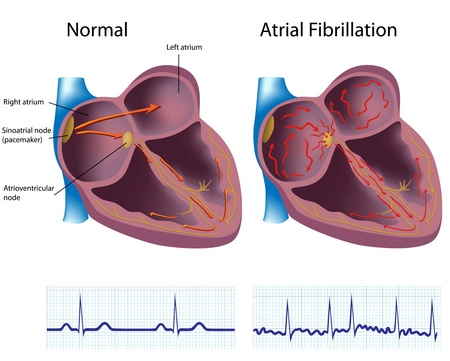
\includegraphics[width=.42\linewidth]{fibrillation.jpg}}
\vspace*{-\baselineskip}

\begin{itemize}
    \item \lenitem{Electrical cardioversion is a medical technique that uses synchronized electrical shocks to restore normal heart rhythm in people with persistent arrhythmia.}

    \item \lenitem{This kind of heart rate problem is usually associated with a disease called atrial fibrillation.}
\end{itemize}
\end{frame}

\subsection{Goals and methods}
\begin{frame}{Goals and methods}
\begin{itemize}
    \item The aim of this paper was to create a classification model that accurately predicts whether the procedure will be successful in the short term, based on data on the clinical picture, other indications, and drug therapy prescribed to patients undergoing it.

    \item The focus was initially on Bayesian networks, a well-known probabilistic graphical model. They, however, proved inferior to other methods of classification and machine learning, such as the random forest classifier and artificial neural networks.
\end{itemize}
\end{frame}

\begin{frame}{Methods (cont.)}
\mbox{}\hfill\raisebox{-\height}[0pt][0pt]{
\includegraphics[width=.42\linewidth]{data.png}}
\vspace*{-\baselineskip}

\begin{itemize}
    \item \lenitem{Fitted models were compared by their accuracy, sensitivity (recall), specificity, and other relevant metrics.}
    \item \lenitem{Extra attention was given to data preprocessing and exploratory analysis, as well as predictor (feature) importance.}
\end{itemize}
\end{frame}

\section{Dataset}
\subsection{Dataset}
\begin{frame}{Dataset}
\begin{itemize}
    \item Dataset consists of 147 unique instances and was obtained from the Pacemaker Center of the Clinical Center of Serbia.

    \item It pertains to electrical cardioversions performed from 2014 to 2019.

    \item Several groups of attributes -- basics (age, sex...), baseline (clinical picture and other indications), drug therapy (and other), cardioversion data, other irrelevant data (patient status after the procedure).
\end{itemize}
\end{frame}

\subsection{Preprocessing}
\begin{frame}{Preprocessing}
\mbox{}\hfill\raisebox{-\height}[0pt][0pt]{
\includegraphics[width=.42\linewidth]{prep.png}}
\vspace*{-\baselineskip}

\begin{itemize}
    \item \lenitem{Dataset contained many irrelevant, mixed and missing values.}

    \item \lenitem{Removed -- cardioversion date, medical record number, number in database...}

    \item \lenitem{Missing values -- special value (-1) and neighborhood mean imputation}

    \item \lenitem{Mixed data types -- numerical transformation (e.g. if column represents number of months, then 2 is OK, but 5mes $\rightarrow$ 5 and 1god $\rightarrow$ 12)}
\end{itemize}
\end{frame}

\subsection{Target class}
\begin{frame}{Target class}
\mbox{}\hfill\raisebox{-\height}[0pt][0pt]{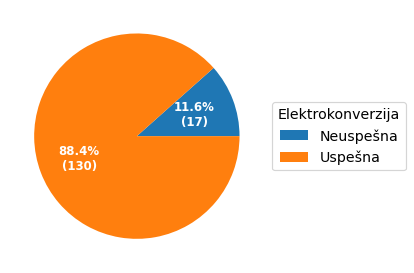
\includegraphics[width=.42\linewidth]{target.png}}
\vspace*{-\baselineskip}

\begin{itemize}
    \item \lenitem{Even though the reccurence rate of atrial fibrillation is very high, most cardioversions are initially successful.}

    \item \lenitem{Successful procedures (88.4 \%) were marked as class True and unsuccessful (11.6 \%) as class False.}
\end{itemize}
\end{frame}

\subsection{Separability}
\begin{frame}{Separability}
\begin{columns}[c]
    \column{.5\textwidth}
    \begin{center}
            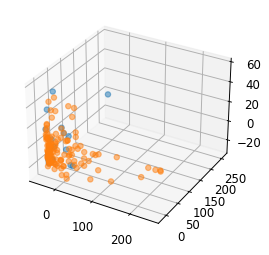
\includegraphics[width=\textwidth]{pca.png}
        \end{center}
    \column{.5\textwidth}
        \begin{center}
             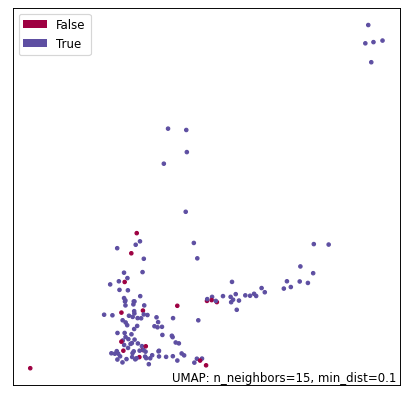
\includegraphics[width=\textwidth]{umap.png} 
        \end{center}
\end{columns}
\end{frame}

\subsection{Feature importance}
\begin{frame}{Feature importance}
\mbox{}\hfill\raisebox{-\height}[0pt][0pt]{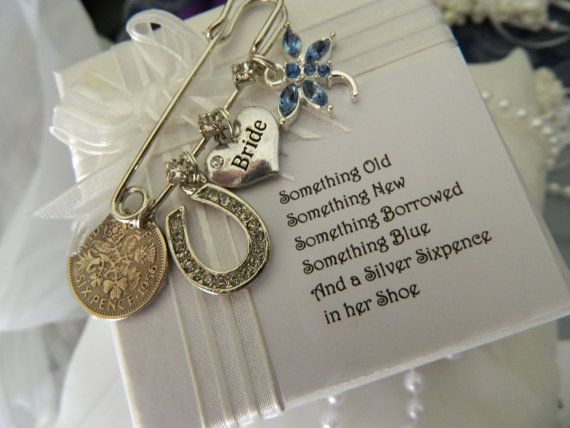
\includegraphics[width=.42\linewidth]{something.jpg}}
\vspace*{-\baselineskip}

\begin{itemize}
    \item Something old:
    \begin{itemize}
        \item domain knowledge -- date irrelevant
    \end{itemize}
    
    \item Something new:
    \begin{itemize}
        \item low correlation with target attribute
        \item high rate of missing values
        \item low variance -- no information
        \item high correlation -- doubled info
    \end{itemize}
    
    \item Something borrowed:
    \begin{itemize}
        \item model predictor importance -- later
    \end{itemize}
    
    \item Something \color{teal}{blue}\color{black}:
    \begin{itemize}
        \item dendrogram and heatmap -- stay tuned
    \end{itemize}
\end{itemize}
\end{frame}

\begin{frame}{Correlation dendrogram}
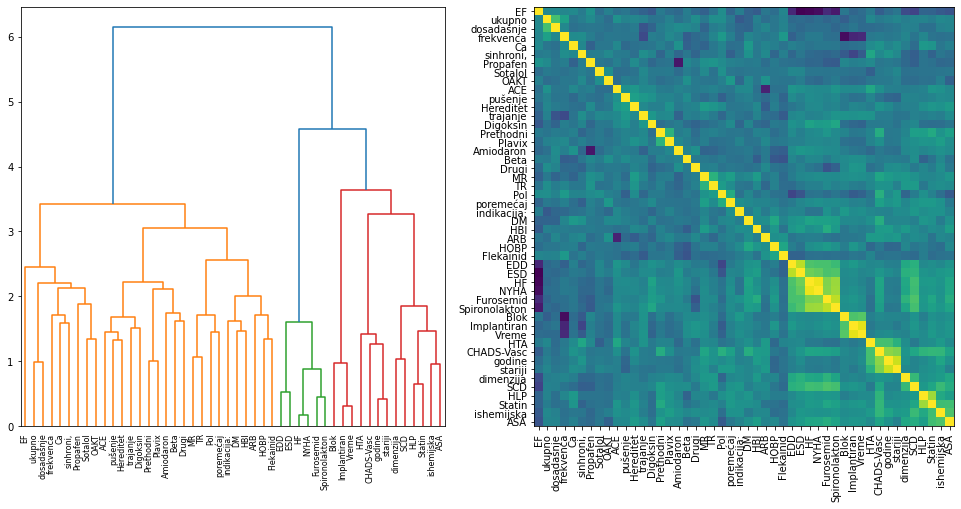
\includegraphics[width=\textwidth]{dendro.png}
\end{frame}

\subsection{To sum up}
\begin{frame}{To sum up}
\begin{itemize}
    \item At the end, dataset dimensions are 147 × 49.

    \item All input variables are of intereger type, with no missing values, while target class is boolean, with somewhat inverted modalities.

    \item Dataset is imbalanced with concern to target class.

    \item This is, of course, a binary classification problem.

    \item According to PCA and UMAP, this seems like a hard problem.
    
    \item It is possible to reduce dimensionality, if needed.
\end{itemize}
\end{frame}

\section{Bayesian networks}
\subsection{Bayesian networks}
\begin{frame}{Bayesian networks}
\begin{itemize}
    \item Bayesian networks are a well-known probabilistic graphical model.
    \item Simply put, BN is a directed acyclic graphs of attributes (vertices), and belief is propagated through its edges.
    \item Discrete form -- each vertex stores conditional probability distribution table of its attribute, given attributes of its parents
    \item Inference -- starts from known attributes, then propagates to target
\end{itemize}
\end{frame}

\subsection{Binning}
\begin{frame}{Binning}
\mbox{}\hfill\raisebox{-\height}[0pt][0pt]{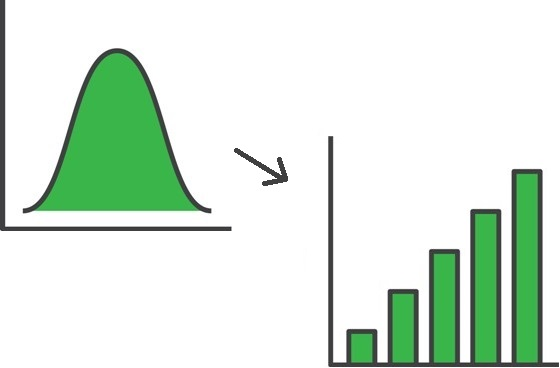
\includegraphics[width=.42\linewidth]{binning.jpeg}}
\vspace*{-\baselineskip}

\begin{itemize}
    \item \lenitem{All data is already discrete; however, it had to be discretized even more to get a good Bayesian network.}

    \item \lenitem{For example, there is only one patient under 30, and his procedure failed. This doesn't mean that youth is a risk factor. Solution -- bin ages $<$ 30, then $30-39$, $40-49$...}
\end{itemize}
\end{frame}

\subsection{Naïve Bayes}
\begin{frame}{Naïve Bayes}
\begin{itemize}
    \item Specific graph structure of the network, such that its branches are directed exclusively from the target to the input attributes.
    \item All such branches exist, and no other.
    \item Implication -- all input variables are independent, given target.
    \item Very simple, but totally underfitted -- every procedure is predicted as successful, which is equal to absolutely naïve (dummy) classifier.
\end{itemize}
\end{frame}

\subsection{Model graph}
\begin{frame}{Model graph}
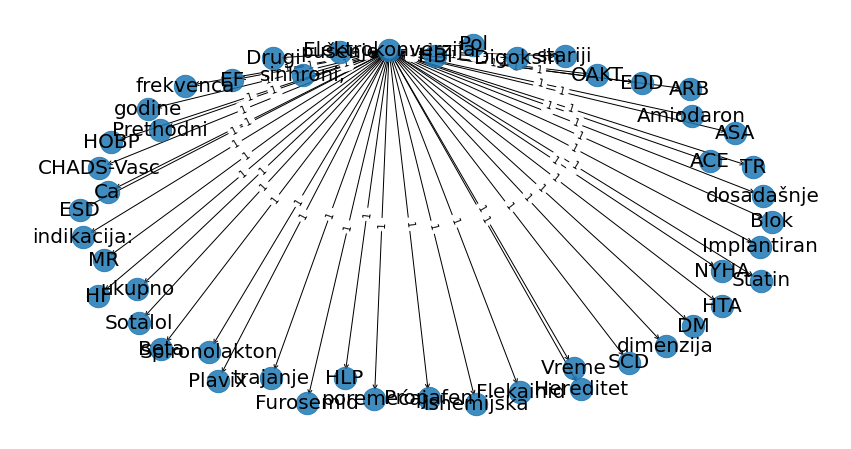
\includegraphics[width=\textwidth]{naive1.png}
\end{frame}

\subsection{Test performance}
\begin{frame}{Test performance}
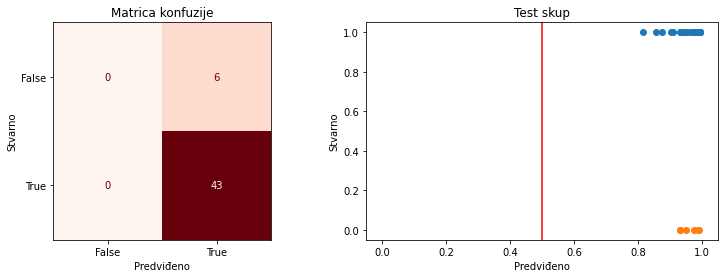
\includegraphics[width=\textwidth]{naive2.png}
\end{frame}

\subsection{Strucutre learning}
\begin{frame}{Strucutre learning}
\begin{itemize}
    \item Hill climbing is used as the optimization techinique for computing the best model graph.
    \item Several scoring measures, including Bayesian information criterion
    \item This model is much better on training partition, but it is still bad at test partition, which means it is overfitted.
\end{itemize}
\end{frame}

\subsection{Model graph}
\begin{frame}{Model graph}
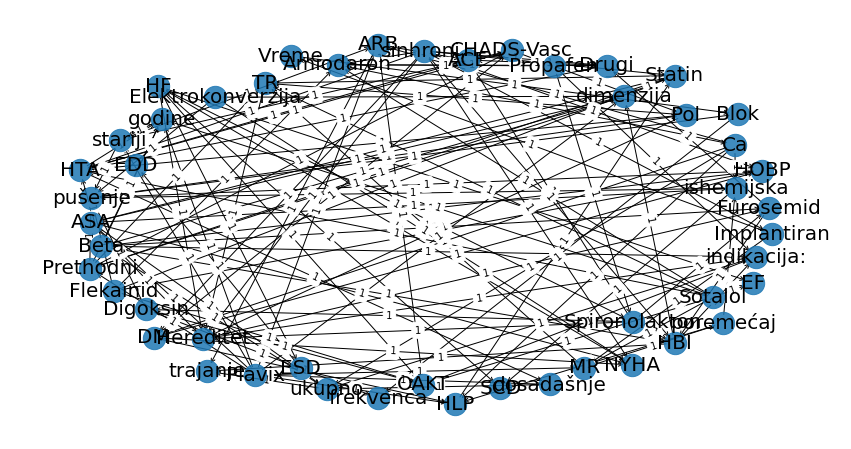
\includegraphics[width=\textwidth]{learn1.png}
\end{frame}

\subsection{Test performance}
\begin{frame}{Test performance}
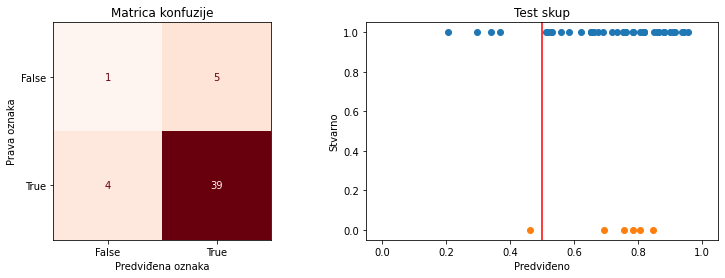
\includegraphics[width=\textwidth]{learn2.png}
\end{frame}

\subsection{Fixed edges}
\begin{frame}{Fixed edges}
\begin{itemize}
    \item Some egdes can be fixed before the start of hill climbing optimization.
    \item It is most sensible to fix edges of type input $\rightarrow$ target.
    \item Model predictor importance (decision tree, random forest...) and dedrogram helped in finding the best combination.
    \item First try -- patient age, heart rate, total duration of the indicated heart disease, ejection fraction
    \item Second try -- heart rate on admission, oral anticoagulant therapy, left atrial diameter, ejection fraction
\end{itemize}
\end{frame}

\subsection{Model graph}
\begin{frame}{Model graph}
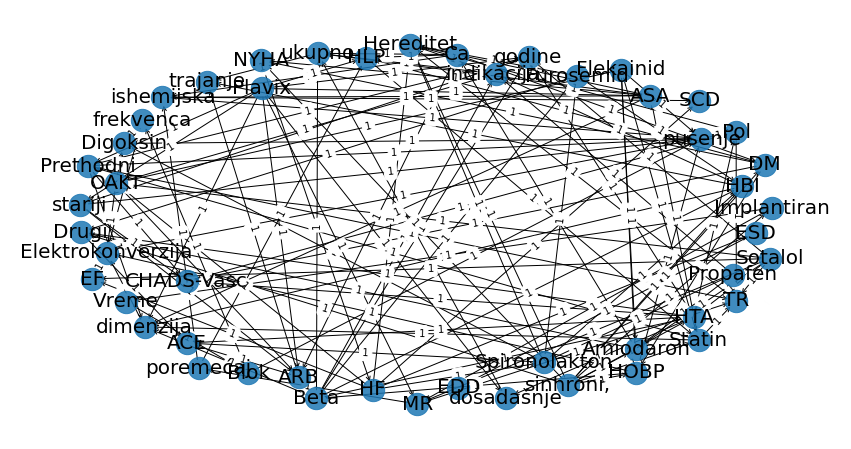
\includegraphics[width=\textwidth]{fixed1.png}
\end{frame}

\subsection{Test performance}
\begin{frame}{Test performance}
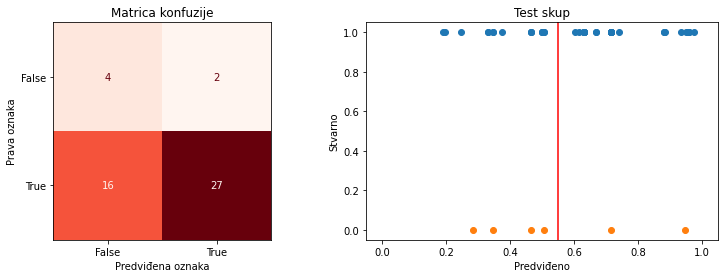
\includegraphics[width=\textwidth]{fixed2.png}
\end{frame}

\section{Other models}
\subsection{Other models}
\begin{frame}{Other models}
\begin{itemize}
    \item Bayesian networks turned out pretty bad.
    \item Luckily, other models saved the day.
    \item Follows: decision trees, support vector machine...
\end{itemize}
\end{frame}

\subsection{Decision tree}
\begin{frame}{Decision tree}
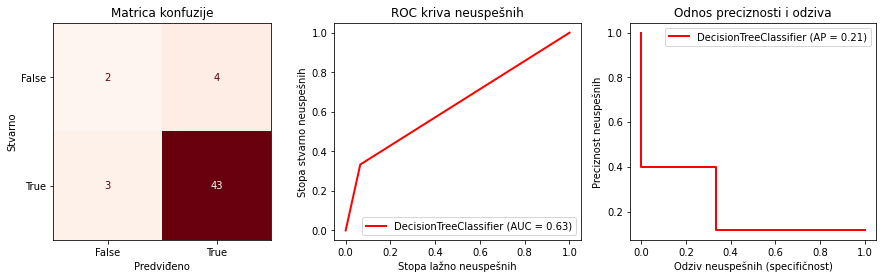
\includegraphics[width=\textwidth]{tree.png}
\end{frame}

\subsection{Tree pruning}
\begin{frame}{Tree pruning}
\begin{center}
    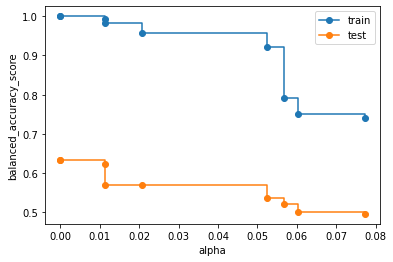
\includegraphics[width=.75\textwidth]{pruning.png}
\end{center}
\end{frame}

\subsection{Complement naïve Bayes}
\begin{frame}{Complement naïve Bayes}
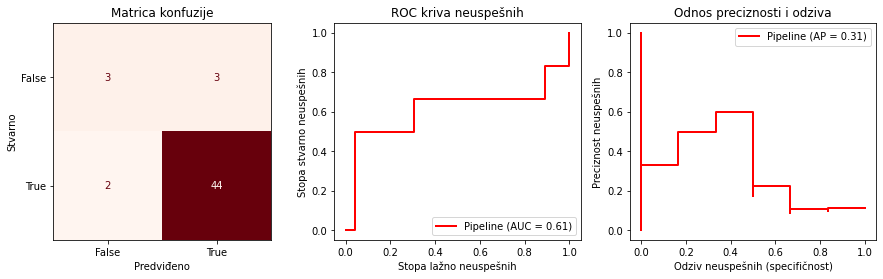
\includegraphics[width=\textwidth]{cnb.png}
\end{frame}

\subsection{Multilayer perceptron}
\begin{frame}{Multilayer perceptron}
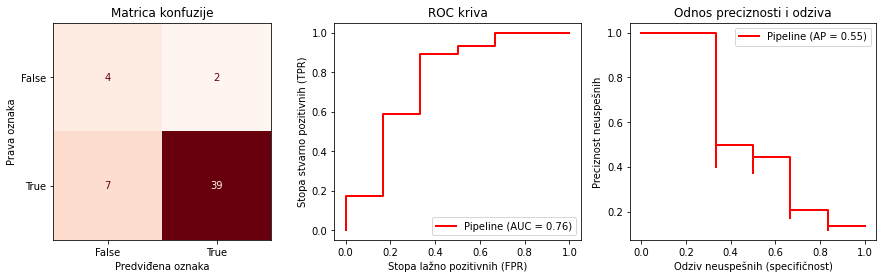
\includegraphics[width=\textwidth]{mlp.png}
\end{frame}

\subsection{Support vector machine}
\begin{frame}{Support vector machine}
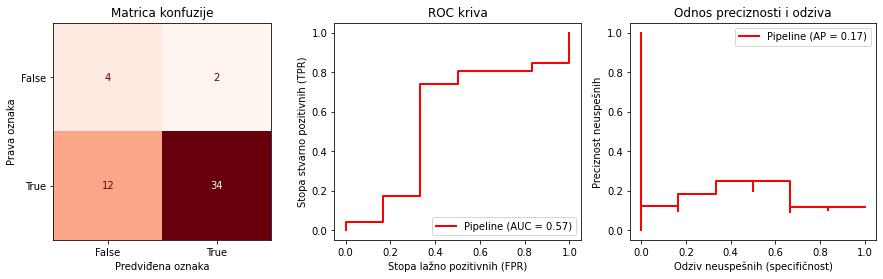
\includegraphics[width=\textwidth]{svm.png}
\end{frame}

\subsection{Ensembles}
\begin{frame}{Ensembles}
\begin{itemize}
    \item Finally, it is possible to combine several models into one.
    \item One way to do so is using simple voting ensembles.
    \item It is best to favorize important unsuccessful procedures.
    \item Dicision function -- conjuction (product) of all input estimators:
    \begin{itemize}
        \item of course, False $\wedge$ False = False,
        \item of course, True $\wedge$ True = True,
        \item also, False $\wedge$ True = False,
        \item also, True $\wedge$ False = False.
    \end{itemize}
\end{itemize}
\end{frame}

\subsection{MLP-SVC ensemble}
\begin{frame}{MLP-SVC ensemble}
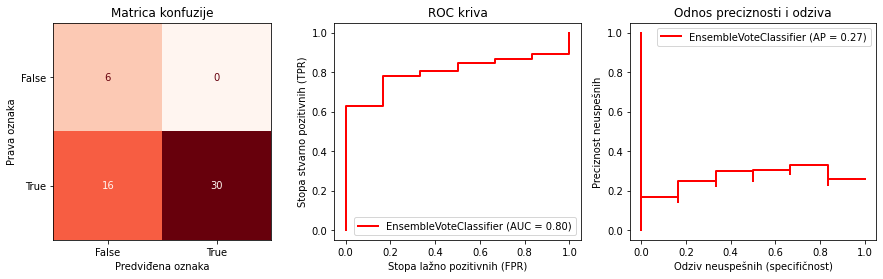
\includegraphics[width=\textwidth]{mlpsvc.png}
\end{frame}

\subsection{RFC-CNB ensemble}
\begin{frame}{RFC-CNB ensemble}
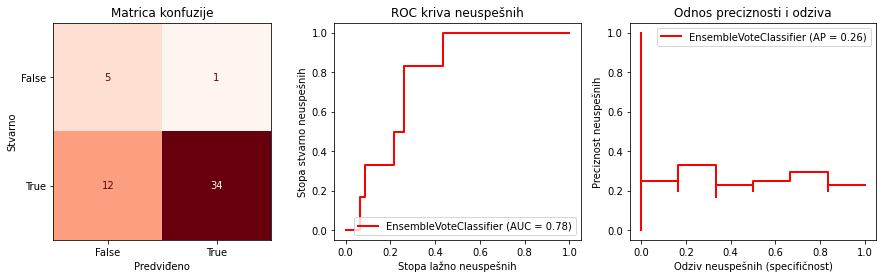
\includegraphics[width=\textwidth]{forcnb.png}
\end{frame}

\subsection{MLP-CNB ensemble}
\begin{frame}{MLP-CNB ensemble}
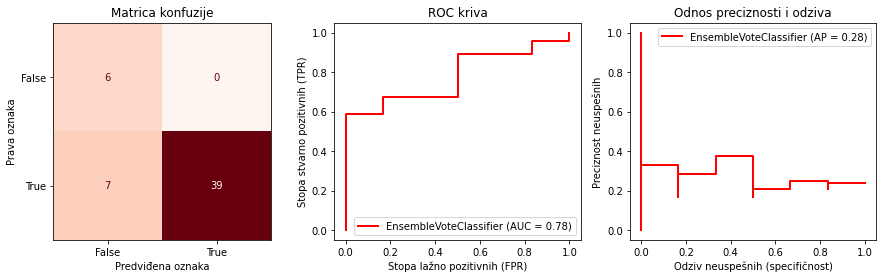
\includegraphics[width=\textwidth]{mlpcnb.png}
\end{frame}

\subsection{MLP-CNB clasification report}
\begin{frame}[fragile]{MLP-CNB clasification report}
\begin{lstlisting}
              precision    recall  f1-score   support

       False       0.46      1.00      0.63         6
        True       1.00      0.85      0.92        46

    accuracy                           0.87        52
   macro avg       0.73      0.92      0.77        52
weighted avg       0.94      0.87      0.88        52
\end{lstlisting}
\end{frame}

\subsection{MLP-CNB pipeline}
\begin{frame}{MLP-CNB pipeline}
\begin{itemize}
    \item Train-test split with augmented train partition
    \begin{itemize}
        \item RandomOverSampler (imblearn)
    \end{itemize}
    
    \item EnsembleVoteClassifier (mlxtend)
    \begin{itemize}
        \item MLPClassifier (sklearn)
        \begin{itemize}
            \item StandardScaler (sklearn)
            \item solver='sgd'
            \item activation='tanh'
            \item hidden\_layer\_sizes=(15, 10)
            \item learning\_rate='invscaling'
            \item learning\_rate\_init=0.001
            \item power\_t=0.6
            \item batch\_size=5
            \item max\_iter=400
        \end{itemize}
        
        \item ComplementNB (sklearn)
        \begin{itemize}
            \item MinMaxScaler (sklearn)
            \item no special parameters
        \end{itemize}
    \end{itemize}
\end{itemize}
\end{frame}

\subsection{MLP-CNB flowchart}
\begin{frame}{MLP-CNB flowchart}
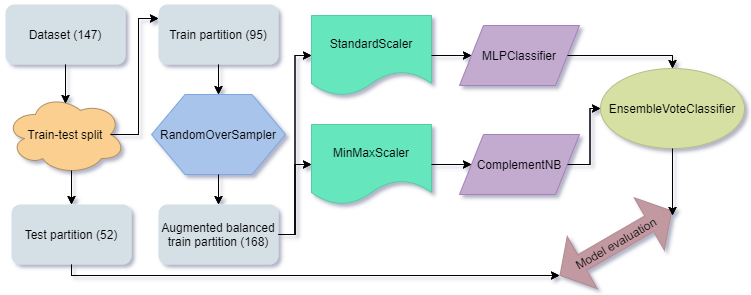
\includegraphics[width=\textwidth]{flowchart.png}
\end{frame}

\section{Conclusion}
\subsection{Conclusion}
\begin{frame}{Conclusion}
\begin{itemize}
    \item All in all, predicting short-term success (immediate outcome) of electrical cardioversion isn't an easy task.
    \item Bayesian networks failed to detect innate dependencies.
    \item Other models were more efficient, with ensembles being the best.
    \item MLP-CNB ensemble managed to score full 100 \% specificity.
    \item Still, precision on important class False is only 46 \%.
\end{itemize}
\end{frame}

\end{document}